\documentclass[tikz,border=8pt]{standalone}
\usepackage[T1]{fontenc}
\usepackage{lmodern}
\usetikzlibrary{arrows.meta,backgrounds,calc,decorations.pathreplacing,fit,positioning}

\definecolor{cpufill}{HTML}{DCEEFF}
\definecolor{cpudraw}{HTML}{2D6EA3}
\definecolor{npufill}{HTML}{FDE6D0}
\definecolor{npudraw}{HTML}{C46B12}
\definecolor{tiledark}{HTML}{F5B16A}
\definecolor{tilelight}{HTML}{FCEBD9}
\definecolor{optionalfill}{HTML}{ECE1FF}
\definecolor{optionaldraw}{HTML}{7F56B3}
\definecolor{routegreen}{HTML}{2F855A}
\definecolor{textgray}{HTML}{5B6470}

\tikzset{
  >={Latex[length=2.7mm,width=1.8mm]},
  basebox/.style={
    rounded corners=4pt,
    draw=black!55,
    line width=0.8pt,
    fill=white,
    align=center,
    minimum height=1.05cm,
    inner sep=5pt,
    font=\small,
  },
  cpubox/.style={basebox, fill=cpufill, draw=cpudraw},
  bodybox/.style={basebox, fill=npufill, draw=npudraw, minimum width=1.55cm},
  optionalbox/.style={basebox, fill=optionalfill, draw=optionaldraw, dashed, minimum width=2.6cm},
  framebox/.style={rounded corners=8pt, draw=black!45, line width=0.9pt},
  tile/.style={
    rounded corners=2pt,
    draw=black!35,
    fill=tilelight,
    minimum width=0.82cm,
    minimum height=0.62cm,
    inner sep=1pt,
    font=\scriptsize\bfseries,
    align=center,
  },
  tilehot/.style={tile, draw=npudraw, line width=0.9pt, fill=tiledark},
  note/.style={font=\scriptsize, text=textgray, align=left},
  notesbox/.style={
    rounded corners=5pt,
    draw=black!20,
    fill=black!3,
    inner sep=6pt,
    align=left,
    font=\scriptsize,
    text width=4.2cm,
  },
}

\begin{document}
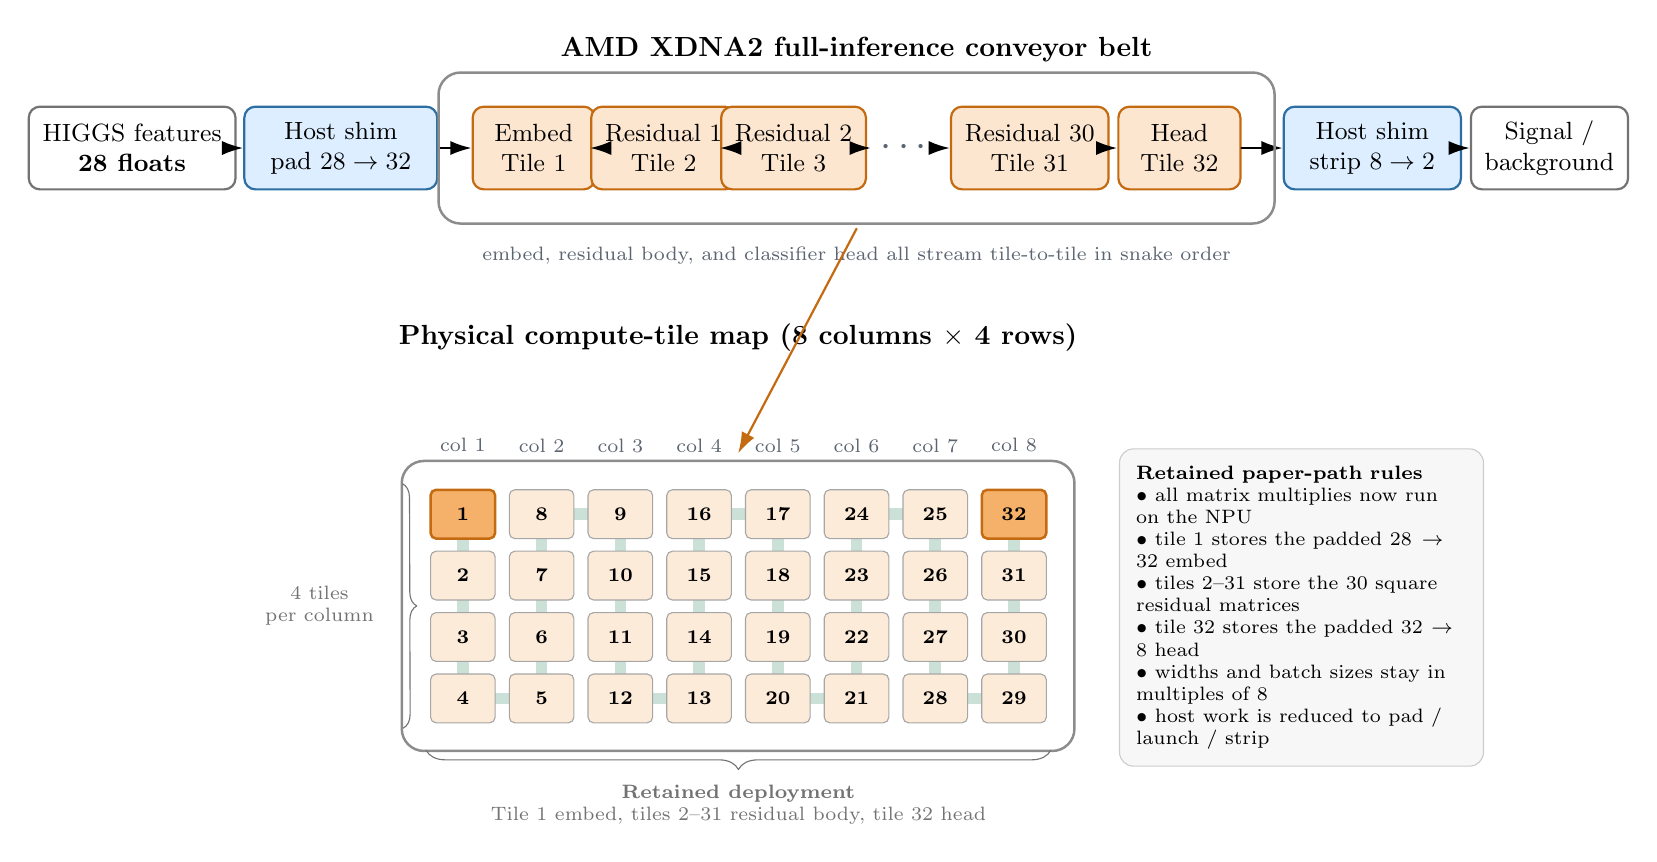
\begin{tikzpicture}[line cap=round, line join=round]
  \node[basebox, minimum width=2.0cm] (input) at (1.25, 6.9) {HIGGS features\\\textbf{28 floats}};
  \node[cpubox, minimum width=2.45cm] (pad) at (3.9, 6.9) {Host shim\\pad $28 \rightarrow 32$};
  \node[bodybox, minimum width=1.55cm] (embed) at (6.35, 6.9) {Embed\\Tile 1};
  \node[bodybox, minimum width=1.55cm] (b1) at (8.0, 6.9) {Residual 1\\Tile 2};
  \node[bodybox, minimum width=1.55cm] (b2) at (9.65, 6.9) {Residual 2\\Tile 3};
  \node[font=\Large, text=textgray] (dots) at (11.05, 6.9) {$\cdots$};
  \node[bodybox, minimum width=1.75cm] (bl) at (12.65, 6.9) {Residual 30\\Tile 31};
  \node[bodybox, minimum width=1.55cm] (headnpu) at (14.55, 6.9) {Head\\Tile 32};
  \node[cpubox, minimum width=2.25cm] (strip) at (17.0, 6.9) {Host shim\\strip $8 \rightarrow 2$};
  \node[basebox, minimum width=1.9cm] (output) at (19.25, 6.9) {Signal /\\background};

  \draw[->, thick] (input) -- (pad);
  \draw[->, thick] (pad) -- (embed);
  \draw[->, thick] (embed) -- (b1);
  \draw[->, thick] (b1) -- (b2);
  \draw[->, thick] (b2) -- (dots);
  \draw[->, thick] (dots) -- (bl);
  \draw[->, thick] (bl) -- (headnpu);
  \draw[->, thick] (headnpu) -- (strip);
  \draw[->, thick] (strip) -- (output);

  \node[framebox, fit=(embed)(b1)(b2)(dots)(bl)(headnpu), inner xsep=0.42cm, inner ysep=0.42cm,
        label={[font=\normalsize\bfseries]above:AMD XDNA2 full-inference conveyor belt}] (bodygroup) {};
  \node[note, anchor=north] at ($(bodygroup.south)+(0,-0.16)$)
    {embed, residual body, and classifier head all stream tile-to-tile in snake order};

  \foreach \col in {0,...,7} {
    \pgfmathtruncatemacro{\colnum}{\col + 1}
    \foreach \row in {0,...,3} {
      \pgfmathtruncatemacro{\isodd}{mod(\col, 2)}
      \ifnum\isodd=0
        \pgfmathtruncatemacro{\blockid}{4*\col + \row + 1}
      \else
        \pgfmathtruncatemacro{\blockid}{4*(\col + 1) - \row}
      \fi
      \pgfmathsetmacro{\x}{5.45 + \col * 1.0}
      \pgfmathsetmacro{\y}{2.25 - \row * 0.78}
      \ifnum\blockid=1
        \node[tilehot] (tile-\col-\row) at (\x, \y) {\blockid};
      \else
        \ifnum\blockid=32
          \node[tilehot] (tile-\col-\row) at (\x, \y) {\blockid};
        \else
          \node[tile] (tile-\col-\row) at (\x, \y) {\blockid};
        \fi
      \fi
    }
    \node[note, anchor=south] at ($(tile-\col-0.north)+(0,0.34)$) {col \colnum};
  }

  \node[framebox, fit=(tile-0-0)(tile-7-3), inner sep=0.35cm] (arraygroup) {};
  \node[font=\normalsize\bfseries, anchor=south] at ($(arraygroup.north)+(0,1.25)$)
    {Physical compute-tile map (8 columns $\times$ 4 rows)};

  \draw[decorate, decoration={brace, amplitude=5pt}, black!55]
    ($(tile-0-0.north west)+(-0.34,0.06)$) --
    ($(tile-0-3.south west)+(-0.34,-0.06)$)
    node[midway, left=7pt, align=center, font=\scriptsize] {4 tiles\\per column};

  \begin{scope}[on background layer]
    \draw[routegreen, line width=4.2pt, opacity=0.25]
      (tile-0-0.center) -- (tile-0-1.center) -- (tile-0-2.center) -- (tile-0-3.center)
      -- (tile-1-3.center) -- (tile-1-2.center) -- (tile-1-1.center) -- (tile-1-0.center)
      -- (tile-2-0.center) -- (tile-2-1.center) -- (tile-2-2.center) -- (tile-2-3.center)
      -- (tile-3-3.center) -- (tile-3-2.center) -- (tile-3-1.center) -- (tile-3-0.center)
      -- (tile-4-0.center) -- (tile-4-1.center) -- (tile-4-2.center) -- (tile-4-3.center)
      -- (tile-5-3.center) -- (tile-5-2.center) -- (tile-5-1.center) -- (tile-5-0.center)
      -- (tile-6-0.center) -- (tile-6-1.center) -- (tile-6-2.center) -- (tile-6-3.center)
      -- (tile-7-3.center) -- (tile-7-2.center) -- (tile-7-1.center) -- (tile-7-0.center);
  \end{scope}

  \draw[->, thick, npudraw]
    ($(bodygroup.south)+(0,-0.05)$) -- ($(arraygroup.north)+(0,0.08)$);

  \draw[decorate, decoration={brace, mirror, amplitude=7pt}, black!55]
    ($(tile-0-3.south west)+(-0.05,-0.34)$) --
    ($(tile-7-3.south east)+(0.05,-0.34)$)
    node[midway, below=9pt, align=center, font=\scriptsize] {\textbf{Retained deployment}\\Tile 1 embed, tiles 2--31 residual body, tile 32 head};

  \node[notesbox, anchor=west] at ($(arraygroup.east)+(0.55,-0.02)$) {
    \textbf{Retained paper-path rules}\\
    $\bullet$ all matrix multiplies now run on the NPU\\
    $\bullet$ tile 1 stores the padded $28 \rightarrow 32$ embed\\
    $\bullet$ tiles 2--31 store the 30 square residual matrices\\
    $\bullet$ tile 32 stores the padded $32 \rightarrow 8$ head\\
    $\bullet$ widths and batch sizes stay in multiples of 8\\
    $\bullet$ host work is reduced to pad / launch / strip
  };
\end{tikzpicture}
\end{document}
